\section{Spark::Sp\-Tuple$<$ N, Real $>$ Class Template Reference}
\label{classSpark_1_1SpTuple}\index{Spark::SpTuple@{Spark::SpTuple}}
{\tt \#include $<$Sp\-Tuple.h$>$}

Inheritance diagram for Spark::Sp\-Tuple$<$ N, Real $>$:\begin{figure}[H]
\begin{center}
\leavevmode
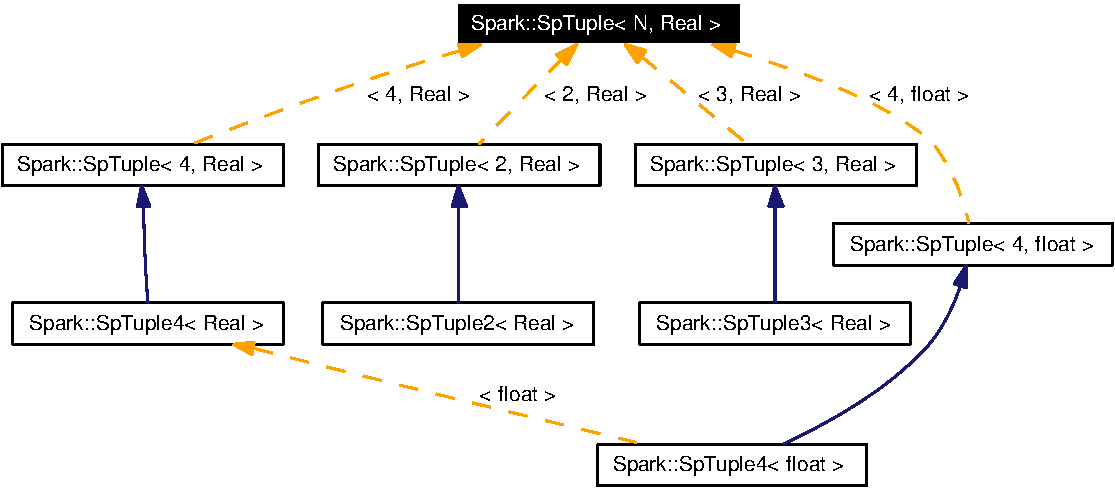
\includegraphics[width=285pt]{classSpark_1_1SpTuple__inherit__graph}
\end{center}
\end{figure}
Collaboration diagram for Spark::Sp\-Tuple$<$ N, Real $>$:\begin{figure}[H]
\begin{center}
\leavevmode
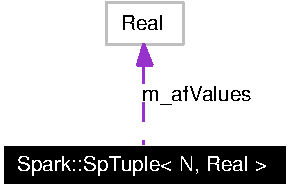
\includegraphics[width=86pt]{classSpark_1_1SpTuple__coll__graph}
\end{center}
\end{figure}


\subsection{Detailed Description}
\subsubsection*{template$<$unsigned int N, class Real$>$ class Spark::Sp\-Tuple$<$ N, Real $>$}

N-Dimensional data class with support for vector mathematics. 

Definition at line 37 of file Sp\-Tuple.h.\subsection*{Public Member Functions}
\begin{CompactItemize}
\item 
{\bf Sp\-Tuple} ()
\begin{CompactList}\small\item\em Construction. \item\end{CompactList}\item 
{\bf Sp\-Tuple} (Real f\-Value)
\item 
{\bf Sp\-Tuple} (const Real $\ast$af\-Sp\-Tuple, unsigned int ui\-N=N)
\item 
{\bf Sp\-Tuple} (const {\bf Sp\-Tuple} \&rk\-V)
\item 
const Real $\ast$ {\bf values} () const
\begin{CompactList}\small\item\em Coordinate Access. \item\end{CompactList}\item 
Real $\ast$ {\bf values} ()
\item 
Real {\bf operator[$\,$]} (unsigned int i) const
\item 
Real \& {\bf operator[$\,$]} (unsigned int i)
\item 
{\bf Sp\-Tuple} \& {\bf operator=} (const {\bf Sp\-Tuple} \&rk\-V)
\begin{CompactList}\small\item\em Assignment:. \item\end{CompactList}\item 
bool {\bf operator==} (const {\bf Sp\-Tuple} \&rk\-V) const
\begin{CompactList}\small\item\em Comparison. \item\end{CompactList}\item 
bool {\bf operator!=} (const {\bf Sp\-Tuple} \&rk\-V) const
\item 
bool {\bf operator$<$} (const {\bf Sp\-Tuple} \&rk\-V) const
\item 
bool {\bf operator$<$=} (const {\bf Sp\-Tuple} \&rk\-V) const
\item 
bool {\bf operator$>$} (const {\bf Sp\-Tuple} \&rk\-V) const
\item 
bool {\bf operator$>$=} (const {\bf Sp\-Tuple} \&rk\-V) const
\item 
{\bf Sp\-Tuple} {\bf operator+} (const {\bf Sp\-Tuple} \&rk\-V) const
\begin{CompactList}\small\item\em Arithmetic:. \item\end{CompactList}\item 
{\bf Sp\-Tuple} {\bf operator-} (const {\bf Sp\-Tuple} \&rk\-V) const
\item 
{\bf Sp\-Tuple} {\bf operator+} (Real f\-Scalar) const
\item 
{\bf Sp\-Tuple} {\bf operator-} (Real f\-Scalar) const
\item 
{\bf Sp\-Tuple} {\bf operator $\ast$} (Real f\-Scalar) const
\item 
{\bf Sp\-Tuple} {\bf operator/} (Real f\-Scalar) const
\item 
{\bf Sp\-Tuple} {\bf operator-} () const
\item 
{\bf Sp\-Tuple} \& {\bf operator+=} (const {\bf Sp\-Tuple} \&rk\-V)
\item 
{\bf Sp\-Tuple} \& {\bf operator-=} (const {\bf Sp\-Tuple} \&rk\-V)
\item 
{\bf Sp\-Tuple} \& {\bf operator+=} (Real f\-Scalar)
\item 
{\bf Sp\-Tuple} \& {\bf operator-=} (Real f\-Scalar)
\item 
{\bf Sp\-Tuple} \& {\bf operator $\ast$=} (Real f\-Scalar)
\item 
{\bf Sp\-Tuple} \& {\bf operator/=} (Real f\-Scalar)
\end{CompactItemize}
\subsection*{Protected Member Functions}
\begin{CompactItemize}
\item 
int {\bf compare} (const {\bf Sp\-Tuple} \&rk\-V) const
\begin{CompactList}\small\item\em Comparison:. \item\end{CompactList}\end{CompactItemize}
\subsection*{Protected Attributes}
\begin{CompactItemize}
\item 
Real {\bf m\_\-af\-Values} [N]
\begin{CompactList}\small\item\em Internal Data:. \item\end{CompactList}\end{CompactItemize}


\subsection{Constructor \& Destructor Documentation}
\index{Spark::SpTuple@{Spark::Sp\-Tuple}!SpTuple@{SpTuple}}
\index{SpTuple@{SpTuple}!Spark::SpTuple@{Spark::Sp\-Tuple}}
\subsubsection{\setlength{\rightskip}{0pt plus 5cm}template$<$unsigned int N, class Real$>$ {\bf Spark::Sp\-Tuple}$<$ N, Real $>$::{\bf Sp\-Tuple} ()}\label{classSpark_1_1SpTuple_a0}


Construction. 

Definition at line 286 of file Sp\-Tuple.h.

References Spark::ivec2, Spark::vec2, Spark::vec3, and Spark::vec4.\index{Spark::SpTuple@{Spark::Sp\-Tuple}!SpTuple@{SpTuple}}
\index{SpTuple@{SpTuple}!Spark::SpTuple@{Spark::Sp\-Tuple}}
\subsubsection{\setlength{\rightskip}{0pt plus 5cm}template$<$unsigned int N, class Real$>$ {\bf Spark::Sp\-Tuple}$<$ N, Real $>$::{\bf Sp\-Tuple} (Real {\em f\-Value})}\label{classSpark_1_1SpTuple_a1}


Definition at line 293 of file Sp\-Tuple.h.

References Spark::bvec2, Spark::bvec3, Spark::bvec4, Spark::ivec3, and Spark::ivec4.\index{Spark::SpTuple@{Spark::Sp\-Tuple}!SpTuple@{SpTuple}}
\index{SpTuple@{SpTuple}!Spark::SpTuple@{Spark::Sp\-Tuple}}
\subsubsection{\setlength{\rightskip}{0pt plus 5cm}template$<$unsigned int N, class Real$>$ {\bf Spark::Sp\-Tuple}$<$ N, Real $>$::{\bf Sp\-Tuple} (const Real $\ast$ {\em af\-Sp\-Tuple}, unsigned int {\em ui\-N} = {\tt N})}\label{classSpark_1_1SpTuple_a2}


Definition at line 299 of file Sp\-Tuple.h.

References Spark::float2, Spark::float3, Spark::float4, Spark::Sp\-Color3b, Spark::Sp\-Color4b, Spark::Sp\-Vector2f, Spark::Sp\-Vector3f, and Spark::Sp\-Vector4f.\index{Spark::SpTuple@{Spark::Sp\-Tuple}!SpTuple@{SpTuple}}
\index{SpTuple@{SpTuple}!Spark::SpTuple@{Spark::Sp\-Tuple}}
\subsubsection{\setlength{\rightskip}{0pt plus 5cm}template$<$unsigned int N, class Real$>$ {\bf Spark::Sp\-Tuple}$<$ N, Real $>$::{\bf Sp\-Tuple} (const {\bf Sp\-Tuple}$<$ N, Real $>$ \& {\em rk\-V})}\label{classSpark_1_1SpTuple_a3}


Definition at line 310 of file Sp\-Tuple.h.

References Spark::Sp\-Color3i, Spark::Sp\-Color3ub, Spark::Sp\-Color4i, and Spark::Sp\-Color4ub.

\subsection{Member Function Documentation}
\index{Spark::SpTuple@{Spark::Sp\-Tuple}!compare@{compare}}
\index{compare@{compare}!Spark::SpTuple@{Spark::Sp\-Tuple}}
\subsubsection{\setlength{\rightskip}{0pt plus 5cm}template$<$unsigned int N, class Real$>$ int {\bf Spark::Sp\-Tuple}$<$ N, Real $>$::compare (const {\bf Sp\-Tuple}$<$ N, Real $>$ \& {\em rk\-V}) const\hspace{0.3cm}{\tt  [protected]}}\label{classSpark_1_1SpTuple_b0}


Comparison:. 

Definition at line 361 of file Sp\-Tuple.h.\index{Spark::SpTuple@{Spark::Sp\-Tuple}!operator *@{operator $\ast$}}
\index{operator *@{operator $\ast$}!Spark::SpTuple@{Spark::Sp\-Tuple}}
\subsubsection{\setlength{\rightskip}{0pt plus 5cm}template$<$unsigned int N, class Real$>$ {\bf Sp\-Tuple}$<$ N, Real $>$ {\bf Spark::Sp\-Tuple}$<$ N, Real $>$::operator $\ast$ (Real {\em f\-Scalar}) const}\label{classSpark_1_1SpTuple_a19}


Definition at line 436 of file Sp\-Tuple.h.\index{Spark::SpTuple@{Spark::Sp\-Tuple}!operator *=@{operator $\ast$=}}
\index{operator *=@{operator $\ast$=}!Spark::SpTuple@{Spark::Sp\-Tuple}}
\subsubsection{\setlength{\rightskip}{0pt plus 5cm}template$<$unsigned int N, class Real$>$ {\bf Sp\-Tuple}$<$ N, Real $>$ \& {\bf Spark::Sp\-Tuple}$<$ N, Real $>$::operator $\ast$= (Real {\em f\-Scalar})}\label{classSpark_1_1SpTuple_a26}


Definition at line 516 of file Sp\-Tuple.h.\index{Spark::SpTuple@{Spark::Sp\-Tuple}!operator"!=@{operator"!=}}
\index{operator"!=@{operator"!=}!Spark::SpTuple@{Spark::Sp\-Tuple}}
\subsubsection{\setlength{\rightskip}{0pt plus 5cm}template$<$unsigned int N, class Real$>$ bool {\bf Spark::Sp\-Tuple}$<$ N, Real $>$::operator!= (const {\bf Sp\-Tuple}$<$ N, Real $>$ \& {\em rk\-V}) const}\label{classSpark_1_1SpTuple_a10}


Definition at line 355 of file Sp\-Tuple.h.\index{Spark::SpTuple@{Spark::Sp\-Tuple}!operator+@{operator+}}
\index{operator+@{operator+}!Spark::SpTuple@{Spark::Sp\-Tuple}}
\subsubsection{\setlength{\rightskip}{0pt plus 5cm}template$<$unsigned int N, class Real$>$ {\bf Sp\-Tuple}$<$ N, Real $>$ {\bf Spark::Sp\-Tuple}$<$ N, Real $>$::operator+ (Real {\em f\-Scalar}) const}\label{classSpark_1_1SpTuple_a17}


Definition at line 418 of file Sp\-Tuple.h.\index{Spark::SpTuple@{Spark::Sp\-Tuple}!operator+@{operator+}}
\index{operator+@{operator+}!Spark::SpTuple@{Spark::Sp\-Tuple}}
\subsubsection{\setlength{\rightskip}{0pt plus 5cm}template$<$unsigned int N, class Real$>$ {\bf Sp\-Tuple}$<$ N, Real $>$ {\bf Spark::Sp\-Tuple}$<$ N, Real $>$::operator+ (const {\bf Sp\-Tuple}$<$ N, Real $>$ \& {\em rk\-V}) const}\label{classSpark_1_1SpTuple_a15}


Arithmetic:. 

Definition at line 400 of file Sp\-Tuple.h.\index{Spark::SpTuple@{Spark::Sp\-Tuple}!operator+=@{operator+=}}
\index{operator+=@{operator+=}!Spark::SpTuple@{Spark::Sp\-Tuple}}
\subsubsection{\setlength{\rightskip}{0pt plus 5cm}template$<$unsigned int N, class Real$>$ {\bf Sp\-Tuple}$<$ N, Real $>$ \& {\bf Spark::Sp\-Tuple}$<$ N, Real $>$::operator+= (Real {\em f\-Scalar})}\label{classSpark_1_1SpTuple_a24}


Definition at line 500 of file Sp\-Tuple.h.\index{Spark::SpTuple@{Spark::Sp\-Tuple}!operator+=@{operator+=}}
\index{operator+=@{operator+=}!Spark::SpTuple@{Spark::Sp\-Tuple}}
\subsubsection{\setlength{\rightskip}{0pt plus 5cm}template$<$unsigned int N, class Real$>$ {\bf Sp\-Tuple}$<$ N, Real $>$ \& {\bf Spark::Sp\-Tuple}$<$ N, Real $>$::operator+= (const {\bf Sp\-Tuple}$<$ N, Real $>$ \& {\em rk\-V})}\label{classSpark_1_1SpTuple_a22}


Definition at line 484 of file Sp\-Tuple.h.\index{Spark::SpTuple@{Spark::Sp\-Tuple}!operator-@{operator-}}
\index{operator-@{operator-}!Spark::SpTuple@{Spark::Sp\-Tuple}}
\subsubsection{\setlength{\rightskip}{0pt plus 5cm}template$<$unsigned int N, class Real$>$ {\bf Sp\-Tuple}$<$ N, Real $>$ {\bf Spark::Sp\-Tuple}$<$ N, Real $>$::operator- () const}\label{classSpark_1_1SpTuple_a21}


Definition at line 466 of file Sp\-Tuple.h.\index{Spark::SpTuple@{Spark::Sp\-Tuple}!operator-@{operator-}}
\index{operator-@{operator-}!Spark::SpTuple@{Spark::Sp\-Tuple}}
\subsubsection{\setlength{\rightskip}{0pt plus 5cm}template$<$unsigned int N, class Real$>$ {\bf Sp\-Tuple}$<$ N, Real $>$ {\bf Spark::Sp\-Tuple}$<$ N, Real $>$::operator- (Real {\em f\-Scalar}) const}\label{classSpark_1_1SpTuple_a18}


Definition at line 427 of file Sp\-Tuple.h.\index{Spark::SpTuple@{Spark::Sp\-Tuple}!operator-@{operator-}}
\index{operator-@{operator-}!Spark::SpTuple@{Spark::Sp\-Tuple}}
\subsubsection{\setlength{\rightskip}{0pt plus 5cm}template$<$unsigned int N, class Real$>$ {\bf Sp\-Tuple}$<$ N, Real $>$ {\bf Spark::Sp\-Tuple}$<$ N, Real $>$::operator- (const {\bf Sp\-Tuple}$<$ N, Real $>$ \& {\em rk\-V}) const}\label{classSpark_1_1SpTuple_a16}


Definition at line 409 of file Sp\-Tuple.h.\index{Spark::SpTuple@{Spark::Sp\-Tuple}!operator-=@{operator-=}}
\index{operator-=@{operator-=}!Spark::SpTuple@{Spark::Sp\-Tuple}}
\subsubsection{\setlength{\rightskip}{0pt plus 5cm}template$<$unsigned int N, class Real$>$ {\bf Sp\-Tuple}$<$ N, Real $>$ \& {\bf Spark::Sp\-Tuple}$<$ N, Real $>$::operator-= (Real {\em f\-Scalar})}\label{classSpark_1_1SpTuple_a25}


Definition at line 508 of file Sp\-Tuple.h.\index{Spark::SpTuple@{Spark::Sp\-Tuple}!operator-=@{operator-=}}
\index{operator-=@{operator-=}!Spark::SpTuple@{Spark::Sp\-Tuple}}
\subsubsection{\setlength{\rightskip}{0pt plus 5cm}template$<$unsigned int N, class Real$>$ {\bf Sp\-Tuple}$<$ N, Real $>$ \& {\bf Spark::Sp\-Tuple}$<$ N, Real $>$::operator-= (const {\bf Sp\-Tuple}$<$ N, Real $>$ \& {\em rk\-V})}\label{classSpark_1_1SpTuple_a23}


Definition at line 492 of file Sp\-Tuple.h.\index{Spark::SpTuple@{Spark::Sp\-Tuple}!operator/@{operator/}}
\index{operator/@{operator/}!Spark::SpTuple@{Spark::Sp\-Tuple}}
\subsubsection{\setlength{\rightskip}{0pt plus 5cm}template$<$unsigned int N, class Real$>$ {\bf Sp\-Tuple}$<$ N, Real $>$ {\bf Spark::Sp\-Tuple}$<$ N, Real $>$::operator/ (Real {\em f\-Scalar}) const}\label{classSpark_1_1SpTuple_a20}


Definition at line 445 of file Sp\-Tuple.h.\index{Spark::SpTuple@{Spark::Sp\-Tuple}!operator/=@{operator/=}}
\index{operator/=@{operator/=}!Spark::SpTuple@{Spark::Sp\-Tuple}}
\subsubsection{\setlength{\rightskip}{0pt plus 5cm}template$<$unsigned int N, class Real$>$ {\bf Sp\-Tuple}$<$ N, Real $>$ \& {\bf Spark::Sp\-Tuple}$<$ N, Real $>$::operator/= (Real {\em f\-Scalar})}\label{classSpark_1_1SpTuple_a27}


Definition at line 524 of file Sp\-Tuple.h.\index{Spark::SpTuple@{Spark::Sp\-Tuple}!operator<@{operator$<$}}
\index{operator<@{operator$<$}!Spark::SpTuple@{Spark::Sp\-Tuple}}
\subsubsection{\setlength{\rightskip}{0pt plus 5cm}template$<$unsigned int N, class Real$>$ bool {\bf Spark::Sp\-Tuple}$<$ N, Real $>$::operator$<$ (const {\bf Sp\-Tuple}$<$ N, Real $>$ \& {\em rk\-V}) const}\label{classSpark_1_1SpTuple_a11}


Definition at line 376 of file Sp\-Tuple.h.\index{Spark::SpTuple@{Spark::Sp\-Tuple}!operator<=@{operator$<$=}}
\index{operator<=@{operator$<$=}!Spark::SpTuple@{Spark::Sp\-Tuple}}
\subsubsection{\setlength{\rightskip}{0pt plus 5cm}template$<$unsigned int N, class Real$>$ bool {\bf Spark::Sp\-Tuple}$<$ N, Real $>$::operator$<$= (const {\bf Sp\-Tuple}$<$ N, Real $>$ \& {\em rk\-V}) const}\label{classSpark_1_1SpTuple_a12}


Definition at line 382 of file Sp\-Tuple.h.\index{Spark::SpTuple@{Spark::Sp\-Tuple}!operator=@{operator=}}
\index{operator=@{operator=}!Spark::SpTuple@{Spark::Sp\-Tuple}}
\subsubsection{\setlength{\rightskip}{0pt plus 5cm}template$<$unsigned int N, class Real$>$ {\bf Sp\-Tuple}$<$ N, Real $>$ \& {\bf Spark::Sp\-Tuple}$<$ N, Real $>$::operator= (const {\bf Sp\-Tuple}$<$ N, Real $>$ \& {\em rk\-V})}\label{classSpark_1_1SpTuple_a8}


Assignment:. 

Definition at line 342 of file Sp\-Tuple.h.\index{Spark::SpTuple@{Spark::Sp\-Tuple}!operator==@{operator==}}
\index{operator==@{operator==}!Spark::SpTuple@{Spark::Sp\-Tuple}}
\subsubsection{\setlength{\rightskip}{0pt plus 5cm}template$<$unsigned int N, class Real$>$ bool {\bf Spark::Sp\-Tuple}$<$ N, Real $>$::operator== (const {\bf Sp\-Tuple}$<$ N, Real $>$ \& {\em rk\-V}) const}\label{classSpark_1_1SpTuple_a9}


Comparison. 

Definition at line 349 of file Sp\-Tuple.h.\index{Spark::SpTuple@{Spark::Sp\-Tuple}!operator>@{operator$>$}}
\index{operator>@{operator$>$}!Spark::SpTuple@{Spark::Sp\-Tuple}}
\subsubsection{\setlength{\rightskip}{0pt plus 5cm}template$<$unsigned int N, class Real$>$ bool {\bf Spark::Sp\-Tuple}$<$ N, Real $>$::operator$>$ (const {\bf Sp\-Tuple}$<$ N, Real $>$ \& {\em rk\-V}) const}\label{classSpark_1_1SpTuple_a13}


Definition at line 388 of file Sp\-Tuple.h.\index{Spark::SpTuple@{Spark::Sp\-Tuple}!operator>=@{operator$>$=}}
\index{operator>=@{operator$>$=}!Spark::SpTuple@{Spark::Sp\-Tuple}}
\subsubsection{\setlength{\rightskip}{0pt plus 5cm}template$<$unsigned int N, class Real$>$ bool {\bf Spark::Sp\-Tuple}$<$ N, Real $>$::operator$>$= (const {\bf Sp\-Tuple}$<$ N, Real $>$ \& {\em rk\-V}) const}\label{classSpark_1_1SpTuple_a14}


Definition at line 394 of file Sp\-Tuple.h.\index{Spark::SpTuple@{Spark::Sp\-Tuple}!operator[]@{operator[]}}
\index{operator[]@{operator[]}!Spark::SpTuple@{Spark::Sp\-Tuple}}
\subsubsection{\setlength{\rightskip}{0pt plus 5cm}template$<$unsigned int N, class Real$>$ Real \& {\bf Spark::Sp\-Tuple}$<$ N, Real $>$::operator[$\,$] (unsigned int {\em i})}\label{classSpark_1_1SpTuple_a7}


Definition at line 335 of file Sp\-Tuple.h.\index{Spark::SpTuple@{Spark::Sp\-Tuple}!operator[]@{operator[]}}
\index{operator[]@{operator[]}!Spark::SpTuple@{Spark::Sp\-Tuple}}
\subsubsection{\setlength{\rightskip}{0pt plus 5cm}template$<$unsigned int N, class Real$>$ Real {\bf Spark::Sp\-Tuple}$<$ N, Real $>$::operator[$\,$] (unsigned int {\em i}) const}\label{classSpark_1_1SpTuple_a6}


Definition at line 328 of file Sp\-Tuple.h.\index{Spark::SpTuple@{Spark::Sp\-Tuple}!values@{values}}
\index{values@{values}!Spark::SpTuple@{Spark::Sp\-Tuple}}
\subsubsection{\setlength{\rightskip}{0pt plus 5cm}template$<$unsigned int N, class Real$>$ Real $\ast$ {\bf Spark::Sp\-Tuple}$<$ N, Real $>$::values ()}\label{classSpark_1_1SpTuple_a5}


Definition at line 322 of file Sp\-Tuple.h.\index{Spark::SpTuple@{Spark::Sp\-Tuple}!values@{values}}
\index{values@{values}!Spark::SpTuple@{Spark::Sp\-Tuple}}
\subsubsection{\setlength{\rightskip}{0pt plus 5cm}template$<$unsigned int N, class Real$>$ const Real $\ast$ {\bf Spark::Sp\-Tuple}$<$ N, Real $>$::values () const}\label{classSpark_1_1SpTuple_a4}


Coordinate Access. 

Definition at line 316 of file Sp\-Tuple.h.

References Spark::Sp\-Color3f, Spark::Sp\-Color3ui, Spark::Sp\-Color4f, and Spark::Sp\-Color4ui.

\subsection{Member Data Documentation}
\index{Spark::SpTuple@{Spark::Sp\-Tuple}!m_afValues@{m\_\-afValues}}
\index{m_afValues@{m\_\-afValues}!Spark::SpTuple@{Spark::Sp\-Tuple}}
\subsubsection{\setlength{\rightskip}{0pt plus 5cm}template$<$unsigned int N, class Real$>$ Real {\bf Spark::Sp\-Tuple}$<$ N, Real $>$::{\bf m\_\-af\-Values}[N]\hspace{0.3cm}{\tt  [protected]}}\label{classSpark_1_1SpTuple_p0}


Internal Data:. 

Definition at line 100 of file Sp\-Tuple.h.

The documentation for this class was generated from the following file:\begin{CompactItemize}
\item 
{\bf Sp\-Tuple.h}\end{CompactItemize}
